\let\negmedspace\undefined
\let\negthickspace\undefined
\documentclass[journal]{IEEEtran}
\usepackage[a5paper, margin=10mm, onecolumn]{geometry}
%\usepackage{lmodern} % Ensure lmodern is loaded for pdflatex
\usepackage{tfrupee} % Include tfrupee package

\setlength{\headheight}{1cm} % Set the height of the header box
\setlength{\headsep}{0mm}     % Set the distance between the header box and the top of the text

\usepackage{gvv-book}
\usepackage{gvv}
\usepackage{cite}
\usepackage{amsmath,amssymb,amsfonts,amsthm}
\usepackage{algorithmic}
\usepackage{graphicx}
\usepackage{textcomp}
\usepackage{xcolor}
\usepackage{txfonts}
\usepackage{listings}
\usepackage{enumitem}
\usepackage{mathtools}
\usepackage{gensymb}
\usepackage{comment}
\usepackage[breaklinks=true]{hyperref}
\usepackage{tkz-euclide} 
\usepackage{listings}
% \usepackage{gvv}                                        
\def\inputGnumericTable{}                                 
\usepackage[latin1]{inputenc}                                
\usepackage{color}                                            
\usepackage{array}                                            
\usepackage{longtable}                                       
\usepackage{calc}                                             
\usepackage{multirow}                                         
\usepackage{hhline}                                           
\usepackage{ifthen}                                           
\usepackage{lscape}
\begin{document}

\bibliographystyle{IEEEtran}
\vspace{3cm}

\title{1.2.14}
\author{EE24BTECH11053 - S A Aravind Eswar
}
% \maketitle
% \newpage
% \bigskip
{\let\newpage\relax\maketitle}

\renewcommand{\thefigure}{\theenumi}
\renewcommand{\thetable}{\theenumi}
\setlength{\intextsep}{10pt} % Space between text and floats


\numberwithin{equation}{enumi}
\numberwithin{figure}{enumi}
\renewcommand{\thetable}{\theenumi}

\textbf{Question:}Verify if the points $\vec{A}\myvec{4\\3}, \vec{B}\myvec{6\\4}, \vec{C}\myvec{5\\-6}\text{ and }\vec{D}\myvec{-3\\5}$ are the vertices of a
parallelogram.\\
\solution 
\begin{table}[h]
	\centering
	\begin{tabular}{|m{5em} | m{7em} | m{10em} |}
    \hline
    \textbf{symbol} & \textbf{Value} & \textbf{Description}\\
    \hline
        \textbf{V},\textbf{u},f & $\myvec{ 1 & 0\\0 & 0}$, $\myvec{0\\2}$, 0 & Parameters of the given conic (parabola)\\
    \hline
        $\vec{h_1}, \vec{m_1}$ & $\myvec{0\\2}, \myvec{1\\0}$ & Parameters of the given line $y = 2$\\
    \hline
        $\vec{h_2}, \vec{m_2}$ & $\myvec{0\\4}, \myvec{1\\0}$ & Parameters of the given line $y = 4$\\
    \hline
        $\vec{a_1}, \vec{a_2}$ & & Points of intersection of given lines to the conic\\
    \hline
        $\kappa_i$ & & Parameters of the line equation $\vec{x} = \vec{h} + \kappa\vec{m}$\\
    \hline
        $A_1$ & & Area under the parabola from $y=0$ to $y=4$\\
    \hline
        $A_2$ & & Area under the parabola from $y=0$ to $y=2$\\
    \hline
\end{tabular}

	\caption{Given Values}
	\label{tab:1}
\end{table}

It requires two vectors formed by two unique points to be equivalent for points $\vec{A},\vec{B},\vec{C}\text{ and }\vec{D}$ to form a parallelogram.
\begin{align}AB = \textbf{B}-\textbf{A} &= \myvec{2\\1}\\BC = \textbf{C}-\textbf{B} &= \myvec{-1\\-10}\\CD =\textbf{D}-\textbf{C} &=\myvec{-8\\11}\\DA = \textbf{A}-\textbf{D} &= \myvec{7\\-2}\\DB = \textbf{D}-\textbf{B} &= \myvec{-9\\1}\\AC = \textbf{C}-\textbf{A} &= \myvec{1\\-9}\end{align}
Thus, the points $\vec{A},\vec{B},\vec{C} \text{ and }\vec{D}$ are not forming a parallelogram.


\begin{figure}[h]
    \centering
    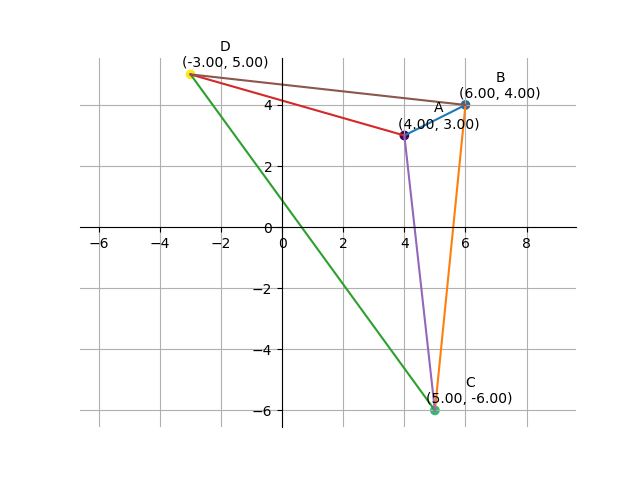
\includegraphics[width=\columnwidth]{figs/fig1.png}
    \caption{Points \textbf{A},\textbf{B},\textbf{C} and \textbf{D}}
 \end{figure}


\end{document}  

